%%%%%%%%%%%%%%%%%%%%%%%%%%%%%%%%%%%%%%
% 
% TODO:
% 1. Figure out a smoother way for the document to flow onto the next page.
% 3. Add more icon options 
% 4. Fix hacky left alignment on contact line
% 5. Remove Hacky fix for awkward extra vertical space
% 
%%%%%%%%%%%%%%%%%%%%%%%%%%%%%%%%%%%%%%
%
% CHANGELOG:
%
%%%%%%%%%%%%%%%%%%%%%%%%%%%%%%%%%%%%%%%
%
% Known Issues:
% 1. Overflows onto second page if any column's contents are more than the vertical limit.
%%%%%%%%%%%%%%%%%%%%%%%%%%%%%%%%%%%%%%
%%Icons:
%%Main: https://icons8.com/icons/carbon-copy
%%%%%%%%%%%%%%%%%%%%%%%%%%%%%%%%%%

\documentclass[]{plushcv}
\usepackage{fancyhdr}
\pagestyle{fancy}
\fancyhf{}
\begin{document}

%%%%%%%%%%%%%%%%%%%%%%%%%%%%%%%%%%%%%%
%
%     MY CV
%
%%%%%%%%%%%%%%%%%%%%%%%%%%%%%%%%%%%%%%

\namesection{Andres}{Acuña Marrroquín}{} 


{\contactline{
\href{mailto:andres.acunamarroquin@gmail.com}{andres.acunamarroquin@gmail.com}}{\href{https://www.github.com/Andres-AM}{Andres-AM}}
{\href{tel:+41782281628}{078 228 16 28}}}
\hfill 
\smash{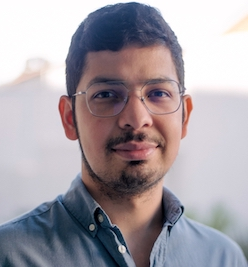
\includegraphics[width=3cm]{Andres.jpeg}}
\sectionsep
\sectionsep
\sectionsep
\sectionsep

%%%%%%%%%%%%%%%%%%%%%%%%%%%%%%%%%%%%%%
%
%     COLUMN ONE
%
%%%%%%%%%%%%%%%%%%%%%%%%%%%%%%%%%%%%%%

\begin{minipage}[t]{0.70\textwidth} 
\sectionsep
\section{PROFILE}
With 4 years of experience in R programming and statistical analysis, my passion lies in applying these skills to understand data and uncover valuable insights. Strong communication abilities complement my technical expertise, enabling effective collaboration and knowledge sharing.

\sectionsep
\sectionsep

\section{TECHNICAL SKILLS}
\begin{tightemize}
\sectionsep
\item Statistics and Machine Learning: I possess expertise in experimental design, t-tests, ANOVA (analysis of variance), time series analysis, regression analysis, and prediction. I am also skilled in sample size calculation and hypothesis testing, allowing me to make informed data-driven decisions.
\item Data Visualization: I excel in presenting data effectively through various techniques, including report writing and creating interactive visualizations using Shiny Apps. This enables autonomous data exploration and enhances the understanding of complex datasets.
\item Bioinformatics: I have experience in conducting DNA database analysis for in silico testing of qPCR probes. Additionally, I am proficient in utilizing server resources and implementing parallel processing techniques to optimize run time for efficient data analysis.
\item Data Quality: I am adept at implementing GAMP5 guidelines, ensuring data quality and compliance. I have a strong focus on automating processes and optimizing data workflows to streamline operations and improve efficiency.
\item Data Wrangling and Version Control: I have extensive experience in data wrangling and utilizing version control systems such as Git and SVN for code management. This ensures proper organization, collaboration, and tracking of changes throughout the data analysis process.
\end{tightemize}

\sectionsep
\sectionsep


%%%%%%%%%%%%%%%%%%%%%%%%%%%%%%%%%%%%%%
%     EXPERIENCE
%%%%%%%%%%%%%%%%%%%%%%%%%%%%%%%%%%%%%%
\sectionsep

\section{WORK EXPERIENCE}

\runsubsection{VERACYTE INC.}
\descript{| Principal Biostatistician }
\location{ May 2019 – August 2022 | Marseille, France}
\begin{tightemize}
\sectionsep
\sectionsep
\item Provided expert statistical counseling to multiple teams/clients involved in the development of qPCR in vitro diagnostic kits. Despite facing overlapping deadlines, I ensured timely completion of projects by effectively managing resources and prioritizing tasks.
\item Conducted comprehensive statistical planning and analysis to evaluate the performance of qPCR kits. As a result, I successfully led the submission of 10 kits compliant with in vitro diagnostic regulations, contributing to the company's regulatory compliance and product success.
\item Demonstrated my technical proficiency by developing three ShinyApps and two R packages. These customized solutions enabled efficient data analysis, including advanced visualization, automated calculations, and reproducibility. By optimizing data analysis processes, I enhanced overall efficiency and productivity.
\item Designed a bioinformatics pipeline specifically tailored for in silico testing of qPCR probes using DNA databases. My focus on process optimization led to significant improvements in efficiency and speed, enabling faster and more accurate testing of probes.
\item Actively participated in the validation of two computerized systems developed in-house, ensuring compliance with GAMP5 guidelines. Through close collaboration with multidisciplinary teams, such as quality insurance and IT, I ensured the robustness and reliability of these systems.
\item As a team leader, I successfully managed and prioritized the tasks of a three-member biostatistics team. By fostering effective communication and leveraging individual strengths, I ensured the timely delivery of high-quality reports and results, promoting overall team success.

\end{tightemize}
\sectionsep
\sectionsep


%%%%%%%%%%%%%%%%%%%%%%%%%%%%%%%%%%%%%%
%
%     COLUMN TWO
%
%%%%%%%%%%%%%%%%%%%%%%%%%%%%%%%%%%%%%%

\end{minipage} 
\hfill
\begin{minipage}[t]{0.25\textwidth} 

\sectionsep
\sectionsep
\sectionsep
\sectionsep


\subsection{Personal details}
\sectionsep
\sectionsep
\sectionsep
\begin{tightemize}
\item Rue du Jura 4 \\ 1201 Genève
\item 07.07.1992  
\item Married
\item Guatemalan
\item B Permit  
\end{tightemize}

\sectionsep


%%%%%%%%%%%%%%%%%%%%%%%%%%%%%%%%%%%%%%
%     SKILLS
%%%%%%%%%%%%%%%%%%%%%%%%%%%%%%%%%%%%%%



\subsection{Programming}
\sectionsep
\runsubsection{}
\justified{ \textbf{I am highly proficient in R programming, with 4 years of experience. I am well-versed in base R, R Shiny, Tidyverse, plotly, package creation, LaTeX, VBA, MATLAB, and SQL. This diverse skill set allows me to handle various data manipulation, analysis, and visualization tasks effectively.}}
\sectionsep

\runsubsection{}
\descript{Libraries/Frameworks}
\justified{ \textbf{Base R \textbullet{}
Tidyverse \textbullet{} R Shiny \textbullet{} plotly \textbullet{} modelr }}
\sectionsep

\runsubsection{}
\descript{Version control}
\justified{ \textbf{Git \textbullet{}SVN}}

\sectionsep

%%%%%%%%%%%%%%%%%%%%%%%%%%%%%%%%%%%%%%
%     EDUCATION
%%%%%%%%%%%%%%%%%%%%%%%%%%%%%%%%%%%%%%
\sectionsep
\subsection{EDUCATION} 
\sectionsep
\descript{MSc. Biomedical engineering | University of Montpellier}
\location{\textbf{2014 - 2016 | France}}
% \justified{\locationthir{Coursework in Reinforcement learning, AI, Data science and Neuroimaging. GPA: 3.85}}

\sectionsep
\descript{BSc. Biotechnologies | University of Montpellier}
\location{2011 - 2014 | France}
% \justified{\locationthir{Relevant coursework completed in statistics and scientific programming.}}
\sectionsep

%%%%%%%%%%%%%%%%%%%%%%%%%%%%%%%%%%%%%%
%     COURSEWORK
%%%%%%%%%%%%%%%%%%%%%%%%%%%%%%%%%%%%%%
\sectionsep
\runsubsection{}
\descript{Coursework}
\justified{ \textbf{ Machine Learning \textbullet{} Artificial Intelligence \textbullet{}
Linux System Administration \textbullet{} 
Visualization For Scientific Data \textbullet{}
Biochemistry \textbullet{}
Genetics \textbullet{}
Cellular biology
}}
\sectionsep
\sectionsep

\end{minipage} 

\clearpage
\begin{minipage}[t]{0.70\textwidth} 
\sectionsep
\sectionsep
\sectionsep
\sectionsep
\sectionsep
\sectionsep
\sectionsep
\sectionsep


%%%%%%%%%%%%%%%%%%%%%%%%%%%%%%%%%%%%%%
%     Page 2
%%%%%%%%%%%%%%%%%%%%%%%%%%%%%%%%%%%%%%

%%%%%%%%%%%%%%%%%%%%%%%%%%%%%%%%%%%%%%
%     Experience
%%%%%%%%%%%%%%%%%%%%%%%%%%%%%%%%%%%%%%


\runsubsection{Institut Image}
\descript{| Statistician }
\location{March 2016 – July 2016 |  Chalon sur Saône, France}
\begin{tightemize}
\sectionsep
\item Designed and implemented a comprehensive evaluation of phobia therapy effectiveness for study participants. This involved developing and executing a robust evaluation methodology.
Conducted thorough statistical analysis to assess the efficacy of the phobia therapy, utilizing appropriate statistical methods to gain a comprehensive understanding of therapy outcomes.
\item Played an active role in participant recruitment for the phobia therapy evaluation, ensuring the formation of a diverse and representative sample to enhance the validity of the study results.
\item Improved the evaluation process by developing a tablet application, resulting in streamlined data acquisition and optimized participant evaluations in terms of efficiency and duration.
\end{tightemize}
\sectionsep


\runsubsection{European Centre for Research on Human Movement}
\descript{| Software Developer (Matlab)}
\location{April 2016 – July 2016 | Montpellier, France}
\begin{tightemize}
\sectionsep
\item Developed a brain-computer interface using an EEG headset to investigate brain wave patterns through time series analysis.
\item Successfully established seamless integration between hardware and software components, facilitating efficient extraction and analysis of signals for a comprehensive understanding of brain wave patterns.
\end{tightemize}

\sectionsep
\sectionsep



% %%%%%%%%%%%%%%%%%%%%%%%%%%%%%%%%%%%%%%
% %     REFERENCES
% %%%%%%%%%%%%%%%%%%%%%%%%%%%%%%%%%%%%%%


\section{REFERENCES} 
\textbf{Olivier Biglia , Associate Director, Technical expert}
\begingroup
\setbox0=\hbox{
\includegraphics[scale=0.1,trim={0 1cm 0cm 0cm}]{icons/main/mail.png}\hspace{0.1cm} olivier.biglia@veracyte.com
}
\parbox{\wd0}{\box0}\endgroup

\sectionsep
\textbf{Régis Perbost, Associate Director Biostatistician/Bioinformatician} 
\begingroup
\setbox0=\hbox{
\includegraphics[scale=0.1,trim={0 1cm 0cm 0cm}]{icons/main/mail.png}\hspace{0.1cm} regis.perbost@veracyte.com
}
\parbox{\wd0}{\box0}\endgroup
\sectionsep

\sectionsep

\end{minipage} 
\hfill
\begin{minipage}[t]{0.25\textwidth} 
\sectionsep
\sectionsep
\sectionsep
\sectionsep
\sectionsep
\sectionsep
\sectionsep
\sectionsep

\subsection{LANGAGES}
\sectionsep
\runsubsection{}
\location{Fluent}
\descript{English | French | Spanish}

\sectionsep
\runsubsection{}
\location{Basic}
\descript{German}
\sectionsep
\sectionsep

\subsection{INTERESTS} 
\sectionsep
\sectionsep
\sectionsep
\begin{tightemize}
\item Hiking and Trekking (GR20, GR7, sections of the GR4, Tour des Aiguilles Rouges)
\item Bikepacking (Nice - Toulouse, Tour of the Geneva Lake) 
\item Restaurant food volunteering at \href{https://carrefour-rue.ch}{\underline{\textit{Carrefour Rue}}}
\end{tightemize}

\end{minipage}
\end{document}  \documentclass[]{article}
